\item[Sigmoid-Funktion] \hfill \\
		\begin{equation}
			f(x) = \frac{1}{1 + e^x} = \frac{e^x}{e^{x + 1}}
			\label{func:Sigmoid}
		\end{equation}
		\begin{equation}
			f'(x) = f(x) * (1 - f(x))
		\end{equation}
		Die mathematische Form der Sigmoid Aktivierungsfunktion ist in Abbildung \ref{sigmoidFunc} zu sehen.
		Sie bildet die reellen Zahlen \(\mathbb{R}\) auf das Intervall \((0,1)\) ab. 
		Für betragsmäßig größer werdende negative Zahlen nähert sich der Rückgabewert \(0\) an,
		ebenso wie für größer werdende positive Zahlen sich der Rückgabewert an \(1\) annähert.

		Die Sigmoid Funktion ist eine historisch häufig genutze Funktion, da sie das Verhalten eines natürlichen Neurons,
		der biologischen Motivation für künstliche Neuronen, gut nachbildet:
		komplette Inaktivität eines Neurons bei Ausgabe 0 bis zum feuern mit maximaler Frequenz bei Ausgabe 1.

		In der Praxis jedoch haben sich einige Nachteile der Sigmoid Funktion gezeigt, weshalb sie quasi nicht mehr genutzt wird.
		Der gewichtigste von diesen ist, dass ihre Ableitung bei großen Beträgen beinah \(0\) ist.
		Dies führt dazu, dass während der Ausführung des Backpropagation-Algorithmus beinah keine Änderungen passieren und dementsprechend das Netz sehr langsam lernt.
		
		\begin{figure}[h]
			\centering
			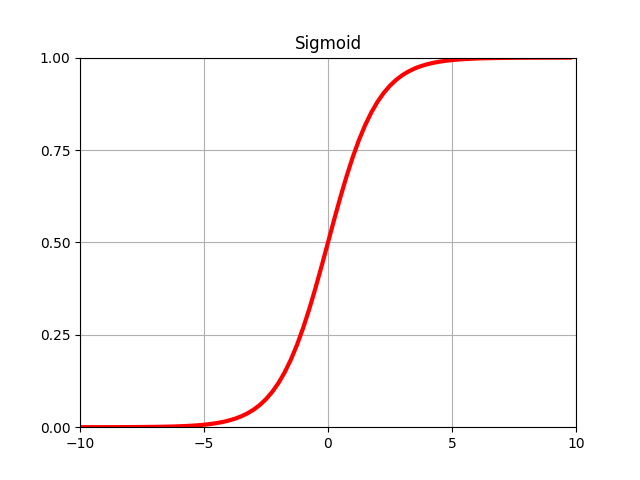
\includegraphics[width=0.618\textwidth]{Sigmoid}
			\caption{Plot der Sigmoid Funktion}
			\label{sigmoidFunc}
		\end{figure}
		  


	\item[TanH] \hfill \\
		\begin{equation}
			f(x) = \tanh(x) = \frac{e^x - e^{-x}}{e^x + e^{-x}}
		\end{equation}
		\begin{equation}
			f'(x) = 1 - f(x)^2
		\end{equation}
		Die TanH-Aktivierungsfunktion ist in Abbildung \ref{tanhfunction} dargestellt.
		Im Gegensatz zur Sigmoid Funktion bildet sie die reellen Zahlen \(\mathbb{R}\) auf das Intervall \((-1, 1)\) ab.
		Weil sie zentriert um den Nullpunkt ist, wird sie bei realen Anwendungen der Sigmoid Funktion vorgezogen.
		Das Saturationsproblem der Sigmoid Funktion besteht jedoch immer noch.
		\begin{figure}[h]
			\centering
			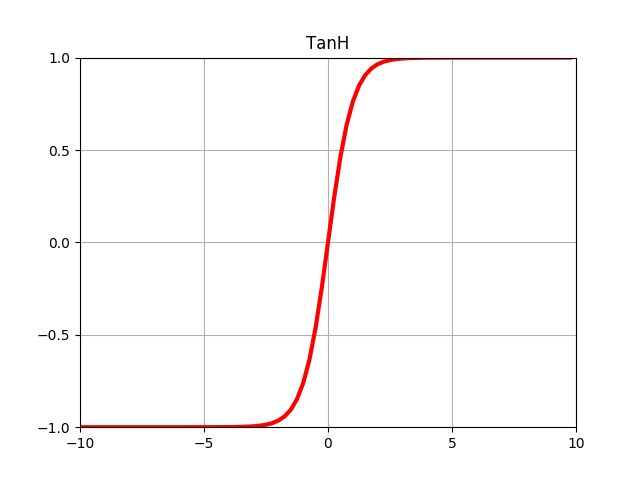
\includegraphics[width=0.618\textwidth]{Tanh}
			\caption{Plot der Tanh Funktion}
			\label{tanhfunction}
		\end{figure}